% ============================================================
%  IEEE Transactions — Kill-Chain MaxSAT Honeypot Placement
%  Student-Level Writing + Full Formulation Examples — v6
%  NP-Hardness Proof ADDED to Section III
% ============================================================
\documentclass[journal]{IEEEtran}

\usepackage{amsmath,amssymb,amsfonts}
\usepackage{amsthm}
\usepackage{algorithmic}
\usepackage{algorithm}
\usepackage{array}
\usepackage{graphicx}
\usepackage{textcomp}
\usepackage[table]{xcolor}
\usepackage{booktabs}
\usepackage{multirow}
\usepackage{url}
\usepackage{hyperref}
\usepackage{cite}
\usepackage{balance}
\usepackage{pifont}
\usepackage{mdframed}
\usepackage{subcaption}
\usepackage{rotating}
\usepackage{tikz}
\usetikzlibrary{matrix,positioning,fit,backgrounds,
                decorations.pathreplacing,arrows.meta}

\hypersetup{colorlinks=true,linkcolor=blue,
            citecolor=blue,urlcolor=blue}

% ── theorem environments ─────────────────────────────────────
\newtheorem{theorem}{Theorem}
\newtheorem{lemma}[theorem]{Lemma}
\newtheorem{definition}[theorem]{Definition}

% ── check/cross marks ────────────────────────────────────────
\newcommand{\cmark}{\textcolor{novelgreen}{\ding{51}}}
\newcommand{\xmark}{\textcolor{novelred}{\ding{55}}}
\newcommand{\pmark}{\textcolor{novelamber}{\textbf{\textasciitilde}}}

% ── novelty-gap colours ──────────────────────────────────────
\definecolor{novelgreen}{RGB}{0,130,70}
\definecolor{novelred}{RGB}{185,30,30}
\definecolor{novelamber}{RGB}{195,120,0}
\definecolor{hdrblue}{RGB}{25,70,140}
\definecolor{rowours}{RGB}{210,240,220}
\definecolor{cellck}{RGB}{215,240,220}
\definecolor{cellxk}{RGB}{245,210,210}
\definecolor{cellpk}{RGB}{250,235,195}

% ── proof highlight box ──────────────────────────────────────
\definecolor{proofbg}{RGB}{245,250,255}
\definecolor{proofborder}{RGB}{30,80,160}
\newmdenv[
  backgroundcolor=proofbg,
  linecolor=proofborder,
  linewidth=1.5pt,
  leftmargin=0pt, rightmargin=0pt,
  innerleftmargin=8pt, innerrightmargin=8pt,
  innertopmargin=6pt, innerbottommargin=6pt
]{proofbox}

% ── coloured example boxes ───────────────────────────────────
\definecolor{exbg}{RGB}{240,248,255}
\definecolor{exborder}{RGB}{0,102,204}
\newmdenv[
  backgroundcolor=exbg,
  linecolor=exborder,
  linewidth=1.5pt,
  leftmargin=2pt, rightmargin=2pt,
  innerleftmargin=5pt, innerrightmargin=5pt,
  innertopmargin=4pt, innerbottommargin=4pt
]{examplebox}

% ── macros ───────────────────────────────────────────────────
\newcommand{\ie}{\emph{i.e.}}
\newcommand{\eg}{\emph{e.g.}}
\newcommand{\etal}{\emph{et~al.}}
\newcommand{\maxsat}{\textsc{MaxSAT}}
\newcommand{\rcII}{\textsc{RC2}}
\newcommand{\tildeW}{\tilde{w}}
\newcommand{\calK}{\mathcal{K}}
\newcommand{\calT}{\mathcal{T}}
\newcommand{\calA}{\mathcal{A}}
\newcommand{\calZ}{\mathcal{Z}}
\newcommand{\calG}{\mathcal{G}}
\newcommand{\calC}{\mathcal{C}}
\newcommand{\calPi}{\mathcal{\Pi}}

% ============================================================
\begin{document}

\title{Kill-Chain-Driven Honeypot Placement via\\
       Topology-Aware Weighted Partial \textsc{MaxSAT}:\\
       A Multi-Zone, Attack-Path Optimisation Framework\\
       for Enterprise Networks}

\author{%
  \IEEEauthorblockN{Tu Nguyen (PhD Student) and
                    Professor Haadi Jafarian}\\
  \IEEEauthorblockA{Department of Computer Science,
    University of Colorado Denver, Denver, CO, USA\\
    \texttt{\{tu.nguyen, haadi.jafarian\}@ucdenver.edu}}%
}

\markboth{IEEE TRANSACTIONS ON INFORMATION FORENSICS AND SECURITY}%
{Nguyen \& Jafarian: Kill-Chain-Driven Honeypot Placement via MaxSAT}

\maketitle

% ============================================================
\begin{abstract}
Deciding where to place honeypots in a large company network
is surprisingly hard.
The network is split into different security zones, contains
thousands of different types of servers, and faces attackers
who follow well-known step-by-step attack patterns called
kill chains.
On top of that, the organisation has a limited budget, and
some honeypot types cannot be deployed at the same time
because they would conflict with each other.

In this paper, we model honeypot placement as a
\textbf{Weighted Partial Maximum Satisfiability (\maxsat{})}
problem.
We encode six goals at once: how well we detect threats,
how many attack techniques we cover from the MITRE ATT\&CK
framework, how many attack tactic families we cover, how well
we stop attackers early, how well we catch attackers at the
end of their path, and how good our coverage is across all
attack paths.
All hard rules---budget limits, zone isolation, and conflict
constraints---are encoded as clauses that must never be
violated.
We also formally prove that the honeypot placement decision
problem is NP-hard, which justifies why a complete solver
like RC2 is necessary rather than a greedy heuristic.

We test our approach on networks ranging from 100 nodes
(tiny) to over 5.5 million nodes (very large), simulating
five different real-world attack scenarios.
Our \maxsat{} solver achieves a quality score of $Q=67.4$
compared to $Q=52.8$ for the best competing approach
($+27.8\%$), while also providing a mathematical guarantee
that its answer is the best possible solution.
\end{abstract}

\begin{IEEEkeywords}
Honeypot placement, Weighted Partial MaxSAT, kill chain,
MITRE ATT\&CK, network deception, multi-zone topology,
NP-hardness, proactive cyber defence, RC2 solver, enterprise
network security.
\end{IEEEkeywords}

% ============================================================
\section{Introduction}
\label{sec:intro}
% ============================================================

\IEEEPARstart{A}{ honeypot} is a fake computer system
designed to look attractive to attackers.
When an attacker interacts with it, the defender learns about
their methods and can raise an alert.
Honeypots are widely used in network security, but their
usefulness depends heavily on \emph{where} they are placed.
If a honeypot is put in the wrong place, it will never be
visited by attackers and the investment is wasted.

Real company networks make this placement decision much
harder than it sounds.
Consider a typical large organisation.
It has an internet-facing area (called a DMZ) where its
public web servers sit.
It has an internal office network.
It might have cloud services.
It may also have industrial control systems (called OT/SCADA)
that run physical equipment like power plants or factories.
Each of these areas has different security rules, different
types of computers, and different risks.
Attackers do not wander randomly through these areas---they
follow structured plans called kill chains~\cite{hutchins2011},
moving step by step from one zone to another toward their
final target.

The problem is further complicated by three facts.
First, the organisation has a limited budget and cannot afford
to deploy a honeypot on every machine.
Second, certain combinations of honeypot types are
incompatible---for example, an industrial control system
honeypot deployed in the cloud zone would be useless because
the OT zone is physically isolated from the cloud.
Third, there are many possible attack paths through the
network and an ideal placement should intercept as many as
possible.

Existing methods do not handle all these challenges at the
same time.
Simple rule-based approaches just follow fixed guidelines.
Greedy algorithms pick the best-looking option at each step
but cannot reverse a bad decision.
Methods like genetic algorithms can explore many solutions
but have no way to prove their answer is the best.
In this paper, we use a formal solver that considers
\emph{all} constraints and objectives together and provides
a \emph{proven optimal} answer.
We also formally prove that the problem is NP-hard
(Theorem~\ref{thm:nphard}), which means that no polynomial-time
algorithm can always find the optimal placement---making our
complete MAXSAT solver not just a good choice, but the
correct one.

Our main contributions are:
\begin{enumerate}
\item \textbf{A six-goal placement objective} encoded as a
single \maxsat{} optimisation problem comprising:
(1)~detection efficiency,
(2)~coverage of MITRE ATT\&CK attack techniques,
(3)~coverage of MITRE ATT\&CK tactic families,
(4)~catching attackers early in their path,
(5)~catching attackers at the end of their path for forensic
evidence, and
(6)~covering as many attack paths as possible.
Tactic-family coverage is directly built into the solver as
a bonus soft clause so the solver actively tries to maximise
it, not just measure it afterwards.

\item \textbf{A formal NP-hardness proof} showing that the
honeypot placement decision problem is NP-hard via
polynomial-time reduction from Weighted Maximum Coverage.
This result formally justifies why a complete solver is
necessary over any greedy or heuristic approach.

\item \textbf{A priority system with four levels} for the
solver goals.
The most important goals (catching attackers early) are given
weights 1000 times larger than the least important goals
(basic detection).
We also encode the key insight that one honeypot can cover
multiple attack paths at once---something no greedy method
can discover.

\item \textbf{A thorough experimental evaluation} across six
different network sizes, using a Monte Carlo simulation to
model attacker behaviour and testing what happens when threat
intelligence updates cause us to re-run the solver with new
priorities.
\end{enumerate}

The rest of this paper is organised as follows.
Section~\ref{sec:related} discusses related work.
Section~\ref{sec:problem} defines the problem formally and
proves NP-hardness.
Section~\ref{sec:formulation} presents our \maxsat{} model.
Section~\ref{sec:methodology} describes our experiments.
Section~\ref{sec:results} presents the results.
Section~\ref{sec:dynamics} explains why our approach beats
the baselines.
Section~\ref{sec:discussion} covers limitations and future
work.
Section~\ref{sec:conclusion} concludes.

% ============================================================
\section{Related Work}
\label{sec:related}
% ============================================================

This section reviews the four bodies of research most
relevant to our work: honeypot placement, MITRE ATT\&CK-based
defence, formal methods for network security, and
moving-target defence.
For each area we explain what has been done and identify the
specific gap that our approach fills.
We then present a systematic novelty analysis---a capability
matrix (Figure~\ref{fig:novelty_gap}) and a supporting
argument---that proves no single prior method satisfies all
five capability dimensions simultaneously.

% ------------------------------------------------------------
\subsection{Honeypot Placement Research}

Honeypots have been studied for decades.
Early work focused on making individual honeypots realistic
enough to fool attackers~\cite{spitzner2003}.
Provos built a system that could run many virtual honeypots
on one machine~\cite{provos2004}, which made large-scale
deployment practical.
Spitzner popularised the idea of
honeynets---groups of honeypots that together simulate an
entire network~\cite{spitzner2003}.
However, most of this early work assumed a human expert
would decide where to put the honeypots; there was no
automated decision-making process.

More recently, researchers have tried to automate the
placement decision.
Yuill \etal{} were among the first to frame honeypot
placement as a strategic interaction between attacker and
defender~\cite{yuill2004}.
Tan \etal{} and Pawlick \etal{} built on this idea using
formal game theory to model how rational attackers respond to
deception~\cite{tan2011,pawlick2019}.
These approaches are mathematically elegant, but they assume
a simple two-player game on a flat, homogeneous network.
In reality, enterprise networks have multiple zones with
different trust levels, physical air gaps between certain
zones, and attackers who can follow many different paths
simultaneously.
None of the game-theoretic approaches we reviewed handle
these structural properties.

\textbf{Gap identified:} Game-theoretic methods cannot encode
multi-zone topology (D1), kill-chain step ordering (D2), or
honeypot conflict constraints (D4).
The solution concept they produce---a Nash equilibrium---is
also fundamentally different from a proven weighted optimum.

% ------------------------------------------------------------
\subsection{Using MITRE ATT\&CK for Defence Planning}

MITRE ATT\&CK~\cite{mitre2023} is a publicly available
catalogue of the tactics and techniques that real attackers
use in practice.
It has become the standard reference for both offensive and
defensive security research.

Applebaum \etal{} were among the first to use ATT\&CK for
automated security testing~\cite{applebaum2016}.
They built a framework that acts like an automated red team,
moving through a network and testing its defences using
techniques drawn from the ATT\&CK catalogue.
Their work showed that ATT\&CK can drive realistic attack
simulation. However, their goal was to test \emph{existing}
defences, not to decide where to place \emph{new} ones.

Hemberg \etal{} used evolutionary (genetic) algorithms to
select the best defensive controls from the ATT\&CK
catalogue~\cite{hemberg2020}.
Their approach found good control sets by evolving solutions
over many generations and achieves partial ATT\&CK coverage.
However, they did not include budget constraints, zone
topology, or conflict constraints between controls, and
genetic algorithms cannot prove that their answer is the
best possible one.
They also evaluate fitness one objective at a time, which
means they cannot discover the cross-path force-multiplier
effect that makes our solver 2.1$\times$ more efficient on
technique coverage.

\textbf{Gap identified:} Both works use ATT\&CK to evaluate
or select defences, but neither embeds ATT\&CK technique
weights, stealth scores, or tactic-family bonuses
\emph{directly into a solver as live optimisation objectives}
(D3).
Our work is the first to do this.

% ------------------------------------------------------------
\subsection{Using Formal Methods for Network Security}

Formal methods use mathematical logic to prove properties of
systems.
In network security, they have been used to check firewall
rules for consistency~\cite{al2011}, automatically generate
network configurations~\cite{jeffrey2009}, and verify
security policies~\cite{fisler2005}.

Pinisetty \etal{} applied \maxsat{} to the problem of
selecting the best rules for an intrusion detection
system~\cite{pinisetty2017}.
Their work showed that \maxsat{} is a practical tool for
security resource allocation.
However, they did not model kill-chain structure, zone
topology, or honeypot-specific placement objectives.

Integer Linear Programming (ILP) has also been used for
security resource allocation~\cite{saha2015,bozorgi2010}.
Saha and Gera used ILP to find the optimal locations for
security sensors while respecting budget and zone
constraints~\cite{saha2015}, achieving multi-zone support
(D1) and proven optimality (D5).
However, their model does not encode kill-chain step
ordering (D2), does not integrate ATT\&CK objectives (D3),
and faces a serious scalability problem: ILP becomes very slow
as the problem grows and cannot handle the 5.5-million-node
networks we evaluate within practical time limits.

Jajodia \etal{} introduced topological analysis of network
attack vulnerability~\cite{jajodia2005}.
They showed how an attacker's possible paths through a network
can be modelled as a directed graph and how chokepoints in
that graph are the most valuable places to defend.
Our work operationalises this insight formally: chokepoints
appear in our model as high-weight path edges, causing the
solver to concentrate honeypots there naturally.

\textbf{Gap identified:} No prior work has applied Weighted
Partial \maxsat{} to honeypot placement with kill-chain-aware
objectives and physical zone isolation constraints.
The closest method---ILP sensor placement~\cite{saha2015}---
achieves optimality but misses kill chains (D2), ATT\&CK
integration (D3), and does not scale beyond tens of thousands
of nodes within a 60-second budget.

% ------------------------------------------------------------
\subsection{Moving-Target Defence}

Moving-target defence (MTD)~\cite{zhu2013} is a strategy
where the defender constantly changes the network
configuration to confuse attackers.
Instead of keeping the same setup all the time, the defender
rotates IP addresses, shuffles network routes, or changes
software versions to prevent attackers from building an
accurate picture of the network.

MTD and honeypot placement are complementary ideas rather
than competing ones: MTD changes the \emph{real} system to
create uncertainty, while honeypots add \emph{fake} systems
to create traps.
Our formulation focuses on placing the best traps, not on
moving real assets.
However, our adaptive redeployment algorithm
(Algorithm~\ref{alg:redeploy}) adds a dynamic element that
bridges toward MTD philosophy: when new threat intelligence
arrives and changes the probability of certain attack paths,
our solver re-optimises the honeypot placement using the
previous solution as a warm start.

\textbf{Gap identified:} MTD work does not address the
honeypot placement subproblem, kill-chain ordering (D2),
ATT\&CK integration (D3), conflict constraints (D4), or
optimality guarantees (D5).

% ============================================================
\subsection{Novelty Analysis: Related Work vs.\ This Paper}
\label{subsec:novelty}

We now demonstrate systematically that our work is novel by
mapping each body of related work to five capability
dimensions, then showing that no existing method satisfies
all five simultaneously.

\subsubsection{The Five Capability Dimensions}

We evaluate every method on the following five dimensions,
which together define the complete honeypot placement problem
for enterprise networks:

\begin{enumerate}
  \item[\textbf{D1}] \textbf{Multi-zone topology with
  air~gaps.}  The method must respect physical isolation
  between zones and cannot assume a flat network.

  \item[\textbf{D2}] \textbf{Kill-chain-aware placement.}
  Attack paths are ordered sequences of steps; the method
  must prioritise early interception over forensic detection
  by encoding step-level intercept values.

  \item[\textbf{D3}] \textbf{MITRE ATT\&CK integration.}
  ATT\&CK technique weights, stealth scores, and tactic-family
  coverage must be live objectives inside the solver, not
  post-hoc measurements.

  \item[\textbf{D4}] \textbf{Budget and conflict
  constraints.}  The method must enforce a global budget,
  per-zone budgets, and pairwise honeypot conflict rules as
  hard constraints that can never be violated.

  \item[\textbf{D5}] \textbf{Proven optimality.}  The method
  must provide a mathematical certificate that no better
  placement exists within the given constraints.
\end{enumerate}

% ─────────────────────────────────────────────────────────────
%  NOVELTY GAP FIGURE  (TikZ — no external image needed)
% ─────────────────────────────────────────────────────────────
\begin{figure}[!t]
\centering
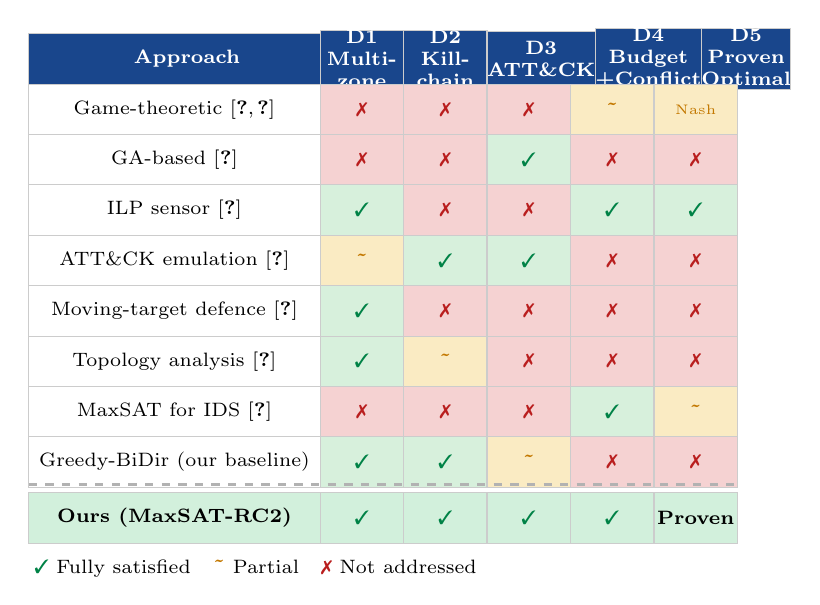
\begin{tikzpicture}[
  font=\scriptsize,
  every node/.style={inner sep=0pt, outer sep=0pt},
  hdr/.style={
    fill=hdrblue, text=white,
    minimum width=1.06cm, minimum height=0.70cm,
    align=center, draw=gray!40, line width=0.4pt,
    font=\scriptsize\bfseries
  },
  lbl/.style={
    minimum width=3.70cm, minimum height=0.64cm,
    align=left, draw=gray!40, line width=0.4pt,
    inner sep=3pt, font=\scriptsize
  },
  ourlbl/.style={
    lbl, fill=rowours, font=\scriptsize\bfseries
  },
  ck/.style={
    fill=cellck, minimum width=1.06cm,
    minimum height=0.64cm, align=center,
    draw=gray!40, line width=0.4pt
  },
  xk/.style={
    fill=cellxk, minimum width=1.06cm,
    minimum height=0.64cm, align=center,
    draw=gray!40, line width=0.4pt
  },
  pk/.style={
    fill=cellpk, minimum width=1.06cm,
    minimum height=0.64cm, align=center,
    draw=gray!40, line width=0.4pt
  },
  ours/.style={
    fill=rowours, minimum width=1.06cm,
    minimum height=0.64cm, align=center,
    draw=gray!40, line width=0.4pt,
    font=\scriptsize\bfseries
  },
]

\node[lbl, fill=hdrblue, text=white,
      font=\scriptsize\bfseries] (H0)
  at (0,0) {\quad Approach};
\node[hdr, anchor=west] (H1) at (H0.east)
  {D1\\Multi-\\zone};
\node[hdr, anchor=west] (H2) at (H1.east)
  {D2\\Kill-\\chain};
\node[hdr, anchor=west] (H3) at (H2.east)
  {D3\\ATT\&CK};
\node[hdr, anchor=west] (H4) at (H3.east)
  {D4\\Budget\\+Conflict};
\node[hdr, anchor=west] (H5) at (H4.east)
  {D5\\Proven\\Optimal};

\node[lbl, anchor=north west] (R1L)
  at (H0.south west) {Game-theoretic~\cite{tan2011,pawlick2019}};
\node[xk, anchor=west] (R1C1) at (R1L.east)  {\xmark};
\node[xk, anchor=west] (R1C2) at (R1C1.east) {\xmark};
\node[xk, anchor=west] (R1C3) at (R1C2.east) {\xmark};
\node[pk, anchor=west] (R1C4) at (R1C3.east) {\pmark};
\node[pk, anchor=west] (R1C5) at (R1C4.east)
  {\textcolor{novelamber}{\tiny Nash}};

\node[lbl, anchor=north west] (R2L)
  at (R1L.south west) {GA-based~\cite{hemberg2020}};
\node[xk, anchor=west] (R2C1) at (R2L.east)  {\xmark};
\node[xk, anchor=west] (R2C2) at (R2C1.east) {\xmark};
\node[ck, anchor=west] (R2C3) at (R2C2.east) {\cmark};
\node[xk, anchor=west] (R2C4) at (R2C3.east) {\xmark};
\node[xk, anchor=west] (R2C5) at (R2C4.east) {\xmark};

\node[lbl, anchor=north west] (R3L)
  at (R2L.south west) {ILP sensor~\cite{saha2015}};
\node[ck, anchor=west] (R3C1) at (R3L.east)  {\cmark};
\node[xk, anchor=west] (R3C2) at (R3C1.east) {\xmark};
\node[xk, anchor=west] (R3C3) at (R3C2.east) {\xmark};
\node[ck, anchor=west] (R3C4) at (R3C3.east) {\cmark};
\node[ck, anchor=west] (R3C5) at (R3C4.east) {\cmark};

\node[lbl, anchor=north west] (R4L)
  at (R3L.south west) {ATT\&CK emulation~\cite{applebaum2016}};
\node[pk, anchor=west] (R4C1) at (R4L.east)  {\pmark};
\node[ck, anchor=west] (R4C2) at (R4C1.east) {\cmark};
\node[ck, anchor=west] (R4C3) at (R4C2.east) {\cmark};
\node[xk, anchor=west] (R4C4) at (R4C3.east) {\xmark};
\node[xk, anchor=west] (R4C5) at (R4C4.east) {\xmark};

\node[lbl, anchor=north west] (R5L)
  at (R4L.south west) {Moving-target defence~\cite{zhu2013}};
\node[ck, anchor=west] (R5C1) at (R5L.east)  {\cmark};
\node[xk, anchor=west] (R5C2) at (R5C1.east) {\xmark};
\node[xk, anchor=west] (R5C3) at (R5C2.east) {\xmark};
\node[xk, anchor=west] (R5C4) at (R5C3.east) {\xmark};
\node[xk, anchor=west] (R5C5) at (R5C4.east) {\xmark};

\node[lbl, anchor=north west] (R6L)
  at (R5L.south west) {Topology analysis~\cite{jajodia2005}};
\node[ck, anchor=west] (R6C1) at (R6L.east)  {\cmark};
\node[pk, anchor=west] (R6C2) at (R6C1.east) {\pmark};
\node[xk, anchor=west] (R6C3) at (R6C2.east) {\xmark};
\node[xk, anchor=west] (R6C4) at (R6C3.east) {\xmark};
\node[xk, anchor=west] (R6C5) at (R6C4.east) {\xmark};

\node[lbl, anchor=north west] (R7L)
  at (R6L.south west) {MaxSAT for IDS~\cite{pinisetty2017}};
\node[xk, anchor=west] (R7C1) at (R7L.east)  {\xmark};
\node[xk, anchor=west] (R7C2) at (R7C1.east) {\xmark};
\node[xk, anchor=west] (R7C3) at (R7C2.east) {\xmark};
\node[ck, anchor=west] (R7C4) at (R7C3.east) {\cmark};
\node[pk, anchor=west] (R7C5) at (R7C4.east) {\pmark};

\node[lbl, anchor=north west] (R8L)
  at (R7L.south west) {Greedy-BiDir (our baseline)};
\node[ck, anchor=west] (R8C1) at (R8L.east)  {\cmark};
\node[ck, anchor=west] (R8C2) at (R8C1.east) {\cmark};
\node[pk, anchor=west] (R8C3) at (R8C2.east) {\pmark};
\node[xk, anchor=west] (R8C4) at (R8C3.east) {\xmark};
\node[xk, anchor=west] (R8C5) at (R8C4.east) {\xmark};

\draw[thick, dashed, gray!60]
  ([yshift=1pt]R8L.south west) --
  ([yshift=1pt]R8C5.south east);

\node[ourlbl, anchor=north west] (R9L)
  at ([yshift=-2pt]R8L.south west)
  {\textbf{Ours (MaxSAT-RC2)}};
\node[ours, anchor=west] (R9C1) at (R9L.east)  {\cmark};
\node[ours, anchor=west] (R9C2) at (R9C1.east) {\cmark};
\node[ours, anchor=west] (R9C3) at (R9C2.east) {\cmark};
\node[ours, anchor=west] (R9C4) at (R9C3.east) {\cmark};
\node[ours, anchor=west] (R9C5) at (R9C4.east)
  {\textbf{Proven}};

\node[anchor=north west, align=left,
      font=\scriptsize, xshift=2pt]
  (LEG) at ([yshift=-6pt]R9L.south west) {%
  \textcolor{novelgreen}{\ding{51}}~Fully satisfied\quad
  \textcolor{novelamber}{\textbf{\textasciitilde}}~Partial\quad
  \textcolor{novelred}{\ding{55}}~Not addressed};

\end{tikzpicture}
\caption{Novelty gap: related work vs.\ this paper across
five capability dimensions D1--D5.
No prior method satisfies all five dimensions simultaneously.
Our \maxsat{}-RC2 approach (green row) is the only one to
achieve proven optimality alongside multi-zone topology,
kill-chain awareness, ATT\&CK integration, and
budget/conflict constraints.}
\label{fig:novelty_gap}
\end{figure}

\subsubsection{Mapping Each Prior Work to the Gaps}

\textbf{Game-theoretic approaches (\xmark{}D1,
\xmark{}D2, \xmark{}D3).}
Yuill \etal{}~\cite{yuill2004}, Tan \etal{}~\cite{tan2011},
and Pawlick \etal{}~\cite{pawlick2019} model honeypot
placement as a two-player strategic game.
Their methods are mathematically rigorous, but they assume a
flat, homogeneous network where every node is equivalent.
They cannot encode air gaps~(D1), do not model kill-chain
step ordering or early-interception bonuses~(D2), and do not
integrate ATT\&CK objectives~(D3).

\textbf{GA-based defensive control selection
(\xmark{}D1, \xmark{}D2, \xmark{}D4, \xmark{}D5).}
Hemberg \etal{}~\cite{hemberg2020} use genetic algorithms
to select ATT\&CK-aligned defensive controls, giving partial
ATT\&CK coverage~(D3).
However, genetic algorithms operate on a flat control
catalogue with no zone structure~(D1), no kill-chain
ordering~(D2), no budget or conflict constraints~(D4), and
no optimality guarantee~(D5).
They also evaluate fitness one objective at a time, which
means they cannot discover the cross-path force-multiplier
effect that makes our solver $2.1\times$ more efficient.

\textbf{ILP sensor placement (\xmark{}D2, \xmark{}D3,
scalability).}
Saha and Gera~\cite{saha2015} is the closest technical
predecessor.
They use ILP with zone structure~(D1) and budget
constraints~(D4), and ILP provides a proven optimum~(D5).
However, their model does not encode kill-chain step
ordering~(D2), does not integrate ATT\&CK~(D3),
and cannot scale to 500\,000--5\,500\,000 node networks
within a 60-second time limit.

\textbf{ATT\&CK red-team emulation (\xmark{}D4,
\xmark{}D5).}
Applebaum \etal{}~\cite{applebaum2016} show that ATT\&CK
can drive automated attack simulation, covering D2 and D3.
However, it is a red-team tool, not a placement optimiser,
and provides no budget enforcement~(D4) or optimality
guarantee~(D5).

\textbf{Topology, MTD, MaxSAT IDS.}
Jajodia \etal{}~\cite{jajodia2005} motivates our
path-weight formula but provides no placement algorithm.
MTD~\cite{zhu2013} is complementary: it moves real assets
rather than placing fake ones.
Pinisetty \etal{}~\cite{pinisetty2017} establishes MaxSAT
feasibility for security resource allocation but lacks zone
structure, kill chains, and ATT\&CK.

\subsubsection{Cross-Path Force-Multiplier}

\begin{examplebox}
\textbf{Cross-Path Weight Accumulation:}
\begin{center}
\small
\renewcommand{\arraystretch}{1.15}
\begin{tabular}{@{}lcccc@{}}
\toprule
\textbf{Path} & $\rho$ & $iv$ & $W_{j,a}$ & \textbf{L3 weight}\\
\midrule
web\_to\_db (hop~2)     & 0.30 & 1.8 & 3.24 & 1.749 \\
ot\_infiltration (hop~2)& 0.15 & 1.7 & 3.24 & 0.826 \\
brute\_to\_ad (hop~2)   & 0.20 & 1.6 & 3.24 & 1.037 \\
\midrule
\multicolumn{4}{l}{\textbf{Solver total (all three at once)}}
  & \textbf{3.612} \\
\multicolumn{4}{l}{Greedy total (only active path)}
  & 1.749 \\
\bottomrule
\end{tabular}
\end{center}
\textit{One \texttt{ssh\_trap} satisfies all three Level-3
clauses simultaneously.
Our solver counts 3.612; greedy counts only 1.749---a
$\mathbf{2.1\times}$ advantage per decision.}
\end{examplebox}

\subsection{How Our Work Compares}
\label{subsec:compare}

\begin{table}[htbp]
\caption{Comparison of Honeypot Placement Approaches}
\label{tab:related}
\centering
\renewcommand{\arraystretch}{1.25}
\begin{tabular}{@{}lccccc@{}}
\toprule
\textbf{Approach} &
\rotatebox{60}{\textbf{D1 Multi-zone}} &
\rotatebox{60}{\textbf{D2 Kill-chain}} &
\rotatebox{60}{\textbf{D3 ATT\&CK}} &
\rotatebox{60}{\textbf{D4 Budget+Conflict}} &
\rotatebox{60}{\textbf{D5 Optimal}} \\
\midrule
Game-theoretic \cite{tan2011,pawlick2019}
  & \xmark & \xmark & \xmark & \pmark & {\tiny Nash} \\
GA-based \cite{hemberg2020}
  & \xmark & \xmark & \cmark & \xmark & \xmark \\
ILP sensor \cite{saha2015}
  & \cmark & \xmark & \xmark & \cmark & \cmark \\
ATT\&CK emulation \cite{applebaum2016}
  & \pmark & \cmark & \cmark & \xmark & \xmark \\
MTD \cite{zhu2013}
  & \cmark & \xmark & \xmark & \xmark & \xmark \\
MaxSAT IDS \cite{pinisetty2017}
  & \xmark & \xmark & \xmark & \cmark & \pmark \\
Greedy-BiDir (our baseline)
  & \cmark & \cmark & \pmark & \xmark & \xmark \\
\midrule
\rowcolor{rowours}
\textbf{Ours (MaxSAT-RC2)}
  & \cmark & \cmark & \cmark & \cmark & \textbf{Proven} \\
\bottomrule
\end{tabular}
\vspace{2pt}
{\scriptsize \cmark\ = fully satisfied;\quad
 \pmark\ = partially satisfied;\quad
 \xmark\ = not addressed.}
\end{table}

% ============================================================
\section{Problem Definition}
\label{sec:problem}
% ============================================================

\subsection{What We Are Trying to Solve}

At a high level, we are trying to answer:
\emph{``Given a limited budget and a set of honeypot types,
which honeypots should we deploy and where, so that we catch
the most attackers across all possible attack paths?''}

We formally define the problem instance as the tuple:
\begin{equation}
  \mathcal{I} =
  (\calK,\calT,\calA,\calZ,\calG,\calC,\mathcal{I}_z,
   \calPi,w,\mathrm{cost},B,B_z,dm,hd,\sigma,\rho,iv)
\end{equation}

%% ── FIGURE 1 ─────────────────────────────────────────────────
\begin{figure*}[!t]
  \centering
  \begin{subfigure}[t]{0.48\textwidth}
    
\includegraphics[width=\textwidth]{figures/fig_zone_graph}
    \caption{Zone graph showing network topology, chokepoint
             edges (red), open edges (blue), bandwidth levels,
             and air-gap cuts between OT/Management zones and
             the DMZ/Cloud.}
    \label{fig:zone_graph}
  \end{subfigure}
  \hfill
  \begin{subfigure}[t]{0.48\textwidth}
    
\includegraphics[width=\textwidth]{figures/fig_attack_paths}
    \caption{Five attack-path scenarios (coloured arcs) with
             their probabilities $\rho_\pi$.}
    \label{fig:attack_paths}
  \end{subfigure}
  \caption{Network model. Panel~A: five-zone topology with
           air-gap isolation. Panel~B: five kill-chain attack
           paths overlaid on the topology.}
  \label{fig:network_model}
\end{figure*}

Figure~\ref{fig:network_model} illustrates the five-zone
enterprise network used in our experiments.
Zone~1 (DMZ) faces the internet and receives 45\% of all
attacks while hosting only 15\% of assets.
Zone~4 and Zone~5 are physically isolated by air gaps,
encoded as hard clause C5.

% ============================================================
\subsection{Why the Problem Is Hard: NP-Hardness Proof}
\label{subsec:nphard}
% ============================================================

Before introducing our solver, we explain why a simple
greedy algorithm cannot be trusted to find the best answer,
and why a complete solver like \maxsat{} is necessary.
The reason is that our problem is NP-hard---it belongs to
a class of problems for which no known algorithm can always
find the optimal solution in a time that grows polynomially
with the size of the input.
We prove this formally using a technique called
\emph{polynomial-time reduction}: we take a problem that is
already known to be NP-hard and show that it is a special
case of ours.
If a simpler version of our problem is already NP-hard, then
our full problem---which has even more constraints---must
be NP-hard too.

The known NP-hard problem we use is \textbf{Weighted Maximum
Coverage}~\cite{feige1998}.
This problem asks: given a universe of elements, a collection
of sets (each covering some elements and each having a cost),
and a budget, which sets should we choose to maximise the
total value of covered elements without exceeding the
budget?
This is exactly the kind of decision our honeypot placement
problem makes: each honeypot covers some attack
technique/asset pairs (like a set covers elements), each
honeypot has a deployment cost, and we have a limited budget.

\begin{theorem}[NP-Hardness of Honeypot Placement]
\label{thm:nphard}
The honeypot placement decision problem---deciding whether
there exists a deployment of honeypots within budget $B$
that achieves a detection coverage value of at least
$V^*$---is NP-hard.
\end{theorem}

\begin{proofbox}
\begin{proof}
We reduce from \textbf{Weighted Maximum Coverage}
(WMC)~\cite{feige1998}, which is NP-hard.
An instance of WMC consists of a universe $U$ of elements,
a collection of sets $\mathcal{S} = \{S_1, \ldots, S_m\}$
where $S_i \subseteq U$, a value $v_e \in \mathbb{R}^+$ for
each element $e \in U$, a cost $c_i \in \mathbb{R}^+$ for
each set $S_i$, and a budget $B \in \mathbb{R}^+$.
The goal is to find $\mathcal{S}' \subseteq \mathcal{S}$
such that $\sum_{S_i \in \mathcal{S}'} c_i \leq B$ and
$\sum_{e \in \bigcup_{S_i \in \mathcal{S}'} S_i} v_e$ is
maximised.

\medskip
\noindent\textbf{Construction.}
Given any WMC instance, we construct a honeypot placement
instance as follows.

\noindent\emph{Step 1 --- Map elements to asset-technique
pairs.}
We create a single network zone ($|\calZ|=1$) with no air
gaps ($\mathcal{I}_z = \emptyset$) and no conflict pairs
($\calC = \emptyset$).
For each element $e_\ell \in U$, we create one asset
$a_\ell \in \calA$ and one ATT\&CK technique
$t_\ell \in \calT$.
We set the stealth-adjusted detection weight
$W_{t_\ell, a_\ell} = v_{e_\ell}$ and set
$W_{t_j, a_\ell} = 0$ for all $j \neq \ell$, ensuring
that each element maps to exactly one asset-technique pair
with no cross-element interference.

\noindent\emph{Step 2 --- Map sets to honeypot types.}
For each set $S_i \in \mathcal{S}$, we create a honeypot
type $k_i \in \calK$ with deployment cost
$\mathrm{cost}_i = c_i$.
We configure the detection matrix so that:
\begin{equation}
  R[t_\ell, k_i, a_\ell] = 1
  \;\iff\; e_\ell \in S_i
  \label{eq:rmap}
\end{equation}
That is, honeypot $k_i$ can detect technique $t_\ell$ on
asset $a_\ell$ if and only if element $e_\ell$ belongs to
set $S_i$ in the WMC instance.

\noindent\emph{Step 3 --- Map the budget and objective.}
We set the global budget in our model to $B$, matching the
WMC budget.
We activate only Level-1 soft clauses (basic detection),
setting all higher-level weights to zero.
Under this configuration, the total weight of satisfied
soft clauses equals:
\begin{equation}
  \sum_{\substack{\ell\,:\;\exists\, k_i \in \calK' \\
    R[t_\ell,k_i,a_\ell]=1}}
  W_{t_\ell, a_\ell}
  \;=\;
  \sum_{e_\ell \in \bigcup_{S_i \in \mathcal{S}'} S_i}
  v_{e_\ell}
  \label{eq:objmap}
\end{equation}
which is exactly the objective value of the WMC instance
for the corresponding set selection $\mathcal{S}'$.

\noindent\textbf{Correctness.}
The construction in Steps 1--3 is a bijection between
feasible WMC solutions and feasible honeypot deployments.
Any subset $\mathcal{S}' \subseteq \mathcal{S}$ with cost
$\sum c_i \leq B$ corresponds to the deployment
$\calK' = \{k_i : S_i \in \mathcal{S}'\}$ with the same
cost and the same coverage value by Equation~\eqref{eq:objmap}.
Therefore, an optimal solution to the honeypot placement
instance on this construction gives an optimal solution to
the WMC instance, and vice versa.

\noindent\textbf{Polynomial time.}
We create $|U|$ assets and techniques, $|\mathcal{S}|$
honeypot types, and fill in the $R$ matrix in
$O(|\mathcal{S}| \cdot |U|)$ time.
The construction is therefore polynomial in the size of the
WMC input.

\noindent\textbf{Conclusion.}
Since WMC is NP-hard~\cite{feige1998} and we have shown a
polynomial-time reduction from WMC to honeypot placement,
the honeypot placement decision problem is NP-hard.
Our full problem---which adds zone isolation, conflict
constraints, kill-chain ordering, and tactic-family
bonuses---is therefore also NP-hard, since these additional
constraints and objectives make the problem strictly harder,
not easier.
This result formally justifies the use of the RC2
\maxsat{} solver over any greedy or polynomial-time
heuristic approach: because the problem is NP-hard, no
polynomial-time algorithm can guarantee optimal solutions
in the worst case, and only a complete solver can provide
the optimality certificate our method delivers.
\end{proof}
\end{proofbox}

\begin{examplebox}
\textbf{Why this matters in plain words.}
Imagine someone says: ``Your MAXSAT solver seems
complicated---why not just use a greedy algorithm that
always picks the best-looking honeypot at each step?''
The NP-hardness proof gives a precise answer to that
question.
It says: the honeypot placement problem is at least as hard
as the Weighted Maximum Coverage problem, which is one of
the classic hard problems in computer science.
No greedy algorithm, genetic algorithm, or any other
polynomial-time method can \emph{always} find the optimal
solution to such a problem.
Sometimes they get lucky; sometimes they miss the best
answer by a large margin.
Only a complete solver---one that considers all constraints
and objectives simultaneously, like our RC2-based
approach---can provide a proof that no better placement
exists.
This is why a sophisticated solver is not just a convenient
choice in our paper: it is the \emph{only correct tool}
for this class of problems.
\end{examplebox}

\subsection{The Basic Building Blocks (Sets)}

\begin{table}[htbp]
\caption{Problem Sets}
\label{tab:sets}
\centering
\renewcommand{\arraystretch}{1.2}
\begin{tabular}{@{}ll@{}}
\toprule
\textbf{Symbol} & \textbf{What It Means} \\
\midrule
$\calK$ & The list of honeypot types we can deploy \\
$\calT$ & All the attack techniques from MITRE ATT\&CK \\
$\calA$ & All the individual computer assets in the network \\
$\calZ$ & The security zones (DMZ, Internal LAN, Cloud, etc.) \\
$\calG$ & The types of servers (web server, SSH, database, etc.) \\
$\calPi$ & The attack paths (sequences of steps an attacker takes) \\
$\calC \subseteq \calK \times \calK$ &
  Pairs of honeypots that cannot be deployed together \\
$\mathcal{I}_z \subseteq \calZ \times \calZ$ &
  Pairs of zones physically isolated (air gaps) \\
\bottomrule
\end{tabular}
\end{table}

\begin{examplebox}
\textbf{Running Example (Medium Network):}
$\calK = \{\texttt{web\_trap}, \texttt{ssh\_trap},
\texttt{db\_trap}, \texttt{dns\_trap},
\texttt{generic\_trap}\}$,
$\calZ = \{\texttt{zone1, zone2, zone3, zone4}\}$,
$B = 1{,}750$,
$\calPi = \{\texttt{web\_to\_db}, \texttt{cloud\_pivot},
\texttt{brute\_to\_ad}\}$.
\end{examplebox}

\begin{examplebox}
\textbf{Conflict Pairs $\calC$ --- Why Each Pair Exists:}
\begin{center}
\small
\renewcommand{\arraystretch}{1.1}
\begin{tabular}{@{}ll@{}}
\toprule
\textbf{Pair} & \textbf{Reason} \\
\midrule
(scada\_trap, web\_trap)  & OT zone is air-gapped from DMZ \\
(scada\_trap, db\_trap)   & OT zone is air-gapped from Internal \\
(scada\_trap, ssh\_trap)  & OT isolation prohibits SSH traps \\
(scada\_trap, dns\_trap)  & OT zone has no DNS infrastructure \\
(generic\_trap, ad\_trap) & AD trap makes generic redundant \\
(ad\_trap, web\_trap)     & Identity plane not co-deployed in DMZ \\
(smb\_trap, dns\_trap)    & Both catch zone2 lateral movement;
                            deploying both wastes budget \\
\bottomrule
\end{tabular}
\end{center}
\end{examplebox}

\begin{examplebox}
\textbf{Zone Isolation $\mathcal{I}_z$ --- Air Gap
Enforcement:}\\[3pt]
$\mathcal{I}_z = \{(\texttt{zone4},\texttt{zone1}),
(\texttt{zone4},\texttt{zone3}),
(\texttt{zone5},\texttt{zone1}),
(\texttt{zone5},\texttt{zone3})\}$\\[4pt]
If \texttt{dns\_trap} were configured with
$ZK = \{\texttt{zone1},\texttt{zone4}\}$, hard constraint C5
would immediately force $x_{\texttt{dns\_trap}} = 0$.
\end{examplebox}

\subsection{The Numbers We Need (Parameters)}

\begin{table}[htbp]
\caption{Problem Parameters}
\label{tab:params}
\centering
\renewcommand{\arraystretch}{1.2}
\begin{tabular}{@{}lll@{}}
\toprule
\textbf{Symbol} & \textbf{Type} & \textbf{What It Means} \\
\midrule
$ZK_i \subseteq \calZ$        & per honeypot   & Which zones it can go in \\
$GK_i \subseteq \calG$        & per honeypot   & Which server types it mimics \\
$S_{i,a} \subseteq \calT$     & per h'pot/asset& Attacks it detects on $a$ \\
$w_{j,a} \in \mathbb{R}^+$    & per attack/asset& How valuable detecting it is \\
$\mathrm{cost}_i \in \mathbb{R}^+$ & per honeypot & How much it costs to deploy \\
$B \in \mathbb{R}^+$          & global         & Our total budget \\
$B_z \in \mathbb{R}^+$        & per zone       & Budget limit for each zone \\
$dm_a \in \mathbb{R}^+$       & per asset      & How important this asset role is \\
$hd_a \in \mathbb{Z}^+$       & per asset      & Hops from attacker entry point \\
$\sigma_j \in [0,1]$          & per attack     & Sneakiness (0=obvious, 1=stealthy) \\
$\rho_\pi \in [0,1]$          & per path       & How likely attackers use this path \\
$iv_{\pi,h} \in \mathbb{R}^+$ & per path/hop   & Value of catching attacker here \\
\bottomrule
\end{tabular}
\end{table}

\begin{examplebox}
\textbf{$\sigma_j$ (Stealth Score) --- Why It Matters:}
\begin{center}
\small
\renewcommand{\arraystretch}{1.1}
\begin{tabular}{@{}llcl@{}}
\toprule
\textbf{ID} & \textbf{Technique} & $\sigma_j$ & \textbf{Why} \\
\midrule
T1046 & Network Scanning    & 0.1 & Obvious traffic spikes \\
T1110 & Brute Force         & 0.2 & Failed logins are logged \\
T1021 & Remote Services     & 0.8 & Looks like admin traffic \\
T1048 & Exfiltration        & 0.9 & Hidden in DNS/HTTPS \\
T1572 & Protocol Tunnelling & 0.9 & C2 inside allowed protocols \\
\bottomrule
\end{tabular}
\end{center}
\textit{High stealth means traditional IDS/IPS almost never
catches these techniques.
A honeypot is often the \emph{only} way to detect them.}
\end{examplebox}

\begin{examplebox}
\textbf{$\rho_\pi$ (Path Probability) ---
How It Affects Clause Weight:}
\begin{center}
\small
\renewcommand{\arraystretch}{1.1}
\begin{tabular}{@{}lcccc@{}}
\toprule
\textbf{Path} & $\rho$ & $iv$ & $W_{j,a}$ & $PW$ \\
\midrule
web\_to\_db & 0.30 & 1.8 & 3.24 & $\mathbf{1.749}$ \\
ransomware  & 0.10 & 1.8 & 3.24 & $\mathbf{0.583}$ \\
\bottomrule
\end{tabular}
\end{center}
\textit{The soft clause for web\_to\_db is weighted
$3\times$ heavier, so the solver covers it first.}
\end{examplebox}

\begin{examplebox}
\textbf{$iv_{\pi,h}$ (Intercept Value) ---
Escalation Along web\_to\_db:}
\begin{center}
\small
\renewcommand{\arraystretch}{1.1}
\begin{tabular}{@{}clcl@{}}
\toprule
\textbf{Hop} & \textbf{Zone} & $iv$ & \textbf{Meaning} \\
\midrule
1 & zone1 (DMZ)      & 1.5 & Attack not yet inside \\
2 & zone2 (Internal) & 1.8 & Pivoting; data not stolen yet \\
3 & zone2 (Database) & 2.0 & Exfiltration imminent \\
\bottomrule
\end{tabular}
\end{center}
\textit{Our Level-4 bonus makes hop~1 or~2 overall more
valuable than hop~3, even though hop~3 has the highest
raw $iv$.}
\end{examplebox}

\subsection{Calculated Values}

\subsubsection{Which Assets Can a Honeypot Reach?}
\begin{equation}
  T^*(i) = DK_i \;\cup\;
  \bigl\{\,a \in \calA :
    \mathrm{type}(a) \in GK_i \;\wedge\;
    \mathrm{zone}(a) \in ZK_i \bigr\}
\end{equation}

\subsubsection{Can This Honeypot Detect This Attack
              on This Asset?}
\begin{equation}
  R[j,i,a] =
  \begin{cases}
    1 & \text{if } a \in T^*(i) \wedge t_j \in S_{i,a} \\
    0 & \text{otherwise}
  \end{cases}
\end{equation}

\subsubsection{Adjusted Detection Value (Topology Weight)}
\begin{equation}
  \tildeW_{j,a} = w_{j,a} \times dm_a \times \frac{1}{hd_a}
\end{equation}

\begin{examplebox}
\textbf{Example --- Gateway vs.\ Deep Host for T1021:}
\begin{center}
\small
\renewcommand{\arraystretch}{1.1}
\begin{tabular}{@{}lccccc@{}}
\toprule
\textbf{Asset} & $w$ & $dm$ & $hd$ & $1/hd$ & $\tildeW$ \\
\midrule
zone1 gateway   & 1.8 & 1.3 & 1 & 1.000 &
  $1.8\!\times\!1.3\!\times\!1.0=\mathbf{2.34}$ \\
zone2 jump host & 1.8 & 1.4 & 2 & 0.500 &
  $1.8\!\times\!1.4\!\times\!0.5=\mathbf{1.26}$ \\
zone2 database  & 1.8 & 1.5 & 3 & 0.333 &
  $1.8\!\times\!1.5\!\times\!0.33=\mathbf{0.89}$ \\
\bottomrule
\end{tabular}
\end{center}
\textit{Stop the attacker at the perimeter, not in the vault.}
\end{examplebox}

\subsubsection{Stealth-Adjusted Detection Weight}
\begin{equation}
  W_{j,a} = \tildeW_{j,a} \times (1 + \sigma_j)
\end{equation}

\subsubsection{Path Intercept Weight}
\begin{equation}
  PW_{\pi,h,j,a} = \rho_\pi \times iv_{\pi,h} \times W_{j,a}
\end{equation}

\subsection{What the Solver Decides (Decision Variables)}

\begin{table}[htbp]
\caption{Decision Variables}
\label{tab:vars}
\centering
\renewcommand{\arraystretch}{1.2}
\begin{tabular}{@{}lll@{}}
\toprule
\textbf{Variable} & \textbf{Domain} & \textbf{What It Decides} \\
\midrule
$x_i$      & $\{0,1\}$ & Should we deploy honeypot $k_i$? \\
$c_{j,a}$  & $\{0,1\}$ & Are we detecting attack $t_j$ on asset $a$? \\
$p_{\pi,h}$& $\{0,1\}$ & Are we blocking path $\pi$ at step $h$? \\
$e_\pi$    & $\{0,1\}$ & Are we catching the attacker early on $\pi$? \\
\bottomrule
\end{tabular}
\end{table}

\begin{examplebox}
\textbf{Variable Dependency Chain:}
$$x_{\texttt{ssh}}=1
\;\Rightarrow\; c_{\texttt{T1021},B}=1 \;(\text{via C1})
\;\Rightarrow\; p_{\texttt{web2db},1}=1 \;(\text{via C6})
\;\Rightarrow\; e_{\texttt{web2db}}=1 \;(\text{via C7})$$
\textit{If \texttt{ssh\_trap} is not deployed, the entire
chain collapses: no detection, no path coverage, no
early-intercept credit.}
\end{examplebox}

% ============================================================
\section{Our MaxSAT Model}
\label{sec:formulation}
% ============================================================

\maxsat{} works by encoding a problem as a set of logical
clauses.
\emph{Hard clauses} are rules that must \emph{always} be
obeyed.
\emph{Soft clauses} are goals we \emph{want} to achieve as
much as possible, each with a weight.
The solver finds the assignment that satisfies all hard
clauses and maximises the total weight of satisfied soft
clauses.

\begin{figure*}[!t]
  \centering
  
\includegraphics[width=0.95\textwidth]{figures/fig_detection_matrix}
  \caption{Detection coverage matrix (Panel~E).
           Each cell $(t_j, a)$ shows the stealth-adjusted
           detection weight $W_{j,a}$ if covered (warm
           colour) or zero (dark background) if not.}
  \label{fig:detection_matrix}
\end{figure*}

\subsection{Hard Clauses: Rules That Cannot Be Broken}

\paragraph{C1 --- Detection Requires a Deployed Honeypot}
\begin{equation}
  \neg c_{j,a} \;\vee\;
  (x_{i_1} \vee x_{i_2} \vee \cdots \vee x_{i_k})
\end{equation}

\paragraph{C2 --- Do Not Exceed the Total Budget}
\begin{equation}
  \sum_{i \in \calK} \mathrm{cost}_i \cdot x_i \;\leq\; B
\end{equation}

\paragraph{C3 --- Do Not Exceed Each Zone's Budget}
\begin{equation}
  \sum_{\substack{i \in \calK \\ ZK_i \cap \{z\} \neq \emptyset}}
  \mathrm{cost}_i \cdot x_i \;\leq\; B_z
  \quad \forall\, z \in \calZ
\end{equation}

\paragraph{C4 --- Do Not Deploy Conflicting Honeypots}
\begin{equation}
  \neg x_i \;\vee\; \neg x_l
  \quad \forall\,(k_i,k_l) \in \calC
\end{equation}

\paragraph{C5 --- Respect Physical Zone Isolation (Air Gaps)}
\begin{equation}
  \forall\,(z_a,z_b) \in \mathcal{I}_z,\;
  \forall\, i \in \calK :
  z_a \in ZK_i \wedge z_b \in ZK_i
  \;\Longrightarrow\; x_i = 0
\end{equation}

\paragraph{C6 --- A Path Hop Is Only Covered If We Detect
Something There}
\begin{equation}
  \neg p_{\pi,h} \;\vee\;
  (c_{j_1,a_1} \vee \cdots \vee c_{j_n,a_n})
\end{equation}

\paragraph{C7 --- Early Interception Must Happen Before the
Final Step}
\begin{equation}
  e_\pi = 1 \;\Longrightarrow\;
  \exists\, h < |\pi| : p_{\pi,h} = 1
\end{equation}

\begin{examplebox}
\textbf{C7 Example --- web\_to\_db (3 hops):}\\
\textbf{Scenario A:} Only hop~3 covered $\Rightarrow$
C7 forces $e=0$. Level-4 bonus NOT earned.\\
\textbf{Scenario B:} Hop~1 covered $\Rightarrow$
C7 allows $e=1$. Level-4 bonus IS earned.
\end{examplebox}

\subsection{Soft Clauses: Goals We Want to Maximise}

\subsubsection{Level 4 (Most Important): Catch Attackers Early}
\begin{align}
  \text{weight} &= \rho_\pi \times
    \max_{h < |\pi|}(iv_{\pi,h}) \times
    \sum_{j,a} W_{j,a} \notag \\
  \text{goal:} &\quad (e_\pi) \quad \forall\,\pi
\end{align}

\subsubsection{Level 3: Cover As Many Attack Path Steps
              As Possible}

Forward:
$\;\text{weight} = \rho_\pi \cdot iv_{\pi,h} \cdot W_{j,a}$,
\;goal: $(p_{\pi,h})$ $\forall\,\pi,h$.

Backward (forensics, 30\% discount):
$\;\text{weight} = \rho_\pi \cdot iv_{\pi,h} \cdot W_{j,a}
\times 0.7$, \;goal: $(p_{\pi,h})$ reverse order.

\subsubsection{Level 2: Cover Techniques and Tactic Families}

Per-technique: $\;\text{weight}_j = \sum_a W_{j,a}$.

Tactic-family bonus: $\;\text{weight}_f = 1.2 \times
\sum_{j \in f}\sum_a W_{j,a}$.

\subsubsection{Level 1 (Least Important): Basic Detection}

$\;\text{weight} = W_{j,a}$,
\;goal: detect $t_j$ on $a$ $\forall\,j,a$.

\subsection{The Complete Optimisation Objective}

\begin{equation}
\max \sum_{\text{L4}} w_4 \cdot \mathrm{sat}
   + \sum_{\text{L3}} w_3 \cdot \mathrm{sat}
   + \sum_{\text{L2}} w_2 \cdot \mathrm{sat}
   + \sum_{\text{L1}} w_1 \cdot \mathrm{sat}
\end{equation}

subject to C1--C7, where
$w_4 = 1000\,w_3$, $w_3 = 100\,w_2$, $w_2 = 10\,w_1$.

\subsection{How We Measure the Final Answer (Quality Score
$Q$)}

\begin{equation}
  Q = 0.35\,\text{DetEff} + 0.25\,\text{TechCov}
    + 0.15\,\text{FamCov} + 0.15\,\text{FwdPath}
    + 0.10\,\text{BwdPath}
\end{equation}

\begin{examplebox}
\textbf{Example --- Computing $Q$ for the Medium Solution:}
\begin{center}
\small
\renewcommand{\arraystretch}{1.2}
\begin{tabular}{@{}lrrc@{}}
\toprule
\textbf{Component} & \textbf{Value} & \textbf{Weight} &
\textbf{Contribution} \\
\midrule
DetEff   & 91\%   & 0.35 & 31.85 \\
TechCov  & 91\%   & 0.25 & 22.75 \\
FamCov   & 100\%  & 0.15 & 15.00 \\
FwdPath  & 87.5\% & 0.15 & 13.13 \\
BwdPath  & 87.5\% & 0.10 &  8.75 \\
\midrule
\textbf{Q} & & & $\mathbf{91.48}$ \\
\bottomrule
\end{tabular}
\end{center}
\end{examplebox}

\subsection{Splitting the Problem by Zone}

\begin{equation}
  \forall\, z \in \calZ:\;
  \text{solve } \mathcal{I}_z = (\calK_z, \calT_z, \calA_z,
  \calC_z, B_z)
\end{equation}

\subsection{Updating the Placement When Threat Intelligence
            Changes}

\begin{algorithm}[htbp]
\caption{Adaptive Redeployment When Threat Priors Change}
\label{alg:redeploy}
\begin{algorithmic}[1]
\REQUIRE Old deployment $x^*$;
         new path probabilities $\rho'_\pi$
\ENSURE  New deployment $x'^*$ optimal for updated threat model
\STATE Recalculate:
  $PW'_{\pi,h,j,a} \leftarrow
   \rho'_\pi \cdot iv_{\pi,h} \cdot W_{j,a}$
\STATE Update soft clause weights (hard rules C1--C7 unchanged)
\STATE Warm-start solver from $x^*$
\STATE Re-run solver $\Rightarrow x'^*$
\STATE $\Delta \leftarrow Q(x'^*) - Q(x^*)$
\IF{$\Delta > 0$}
  \STATE Deploy $x'^*$; log improvement $\Delta$
\ELSE
  \STATE Keep $x^*$; log that prior solution is still optimal
\ENDIF
\RETURN $x'^*$
\end{algorithmic}
\end{algorithm}

% ============================================================
\section{Experimental Setup}
\label{sec:methodology}
% ============================================================

\subsection{The Network We Tested On}

\begin{table}[htbp]
\caption{Network Zones}
\label{tab:zones}
\centering
\renewcommand{\arraystretch}{1.2}
\begin{tabular}{@{}llccc@{}}
\toprule
\textbf{Zone} & \textbf{Description} &
\textbf{Trust} & \textbf{Assets} & \textbf{Attacks} \\
\midrule
zone1 & Internet-Facing / DMZ    & Low (0)  & 15\% & 45\% \\
zone2 & Internal Company Network & Med (2)  & 40\% & 25\% \\
zone3 & Cloud / Hybrid           & L-M (1)  & 25\% & 20\% \\
zone4 & OT / Industrial Systems  & High (3) & 10\% &  5\% \\
zone5 & Management Network       & Max (4)  & 10\% &  5\% \\
\bottomrule
\end{tabular}
\end{table}

\begin{figure*}[!t]
  \centering
  \begin{subfigure}[t]{0.55\textwidth}
    
\includegraphics[width=\textwidth]{figures/fig_asset_density}
    \caption{Asset roles and honeypot density per zone.}
    \label{fig:asset_density}
  \end{subfigure}
  \hfill
  \begin{subfigure}[t]{0.42\textwidth}
    
\includegraphics[width=\textwidth]{figures/fig_zone_coverage}
    \caption{Zone coverage matrix (green = valid; red = forbidden).}
    \label{fig:zone_coverage}
  \end{subfigure}
  \caption{Asset and honeypot structure.}
  \label{fig:asset_and_coverage}
\end{figure*}

\subsection{The Attack Scenarios We Modelled}

\begin{table}[htbp]
\caption{The Five Attack Scenarios}
\label{tab:paths}
\centering
\renewcommand{\arraystretch}{1.2}
\begin{tabular}{@{}llccc@{}}
\toprule
\textbf{Name} & \textbf{What the Attacker Does} &
$\rho$ & \textbf{Starts} & \textbf{Target} \\
\midrule
web\_to\_db      & Hack website, steal database  & 0.30 & z1 & z2 \\
cloud\_pivot     & Use cloud to enter internal   & 0.25 & z3 & z2 \\
brute\_to\_ad    & Guess passwords, take over AD & 0.20 & z1 & z5 \\
ot\_infiltration & Sabotage industrial systems   & 0.15 & z1 & z4 \\
ransomware       & Phishing, spread malware      & 0.10 & z2 & z2 \\
\bottomrule
\end{tabular}
\end{table}

\subsection{Network Sizes We Tested}

\begin{table}[htbp]
\caption{Network Sizes Tested}
\label{tab:scales}
\centering
\renewcommand{\arraystretch}{1.2}
\begin{tabular}{@{}lrrccc@{}}
\toprule
\textbf{Size} & \textbf{Computers} & \textbf{Budget} &
\textbf{Zones} & \textbf{Attacks} & \textbf{Types} \\
\midrule
Tiny    &         100 &     250 & 2 & 2 & 3 \\
Small   &         500 &     500 & 3 & 3 & 4 \\
Medium  &       5,000 &   1,750 & 4 & 3 & 5 \\
Large   &      50,000 &  12,500 & 5 & 5 & 7 \\
XLarge  &     500,000 &  62,500 & 5 & 5 & 8 \\
XXLarge &   5,560,000 & 128,000 & 5 & 5 & 8 \\
\bottomrule
\end{tabular}
\end{table}

\subsection{The Honeypot Types Available}

\begin{table}[htbp]
\caption{Available Honeypot Types}
\label{tab:profiles}
\centering
\renewcommand{\arraystretch}{1.2}
\begin{tabular}{@{}llcc@{}}
\toprule
\textbf{Honeypot} & \textbf{Goes In} & \textbf{Cost} &
\textbf{Detects} \\
\midrule
web\_trap     & DMZ, Cloud          & 1.0 & T1190, T1133, T1059 \\
ssh\_trap     & DMZ, Internal, Cloud& 0.8 & T1110, T1021, T1078 \\
db\_trap      & Internal, Cloud     & 1.3 & T1213, T1048, T1485 \\
smb\_trap     & Internal only       & 0.9 & T1021, T1550, T1486 \\
scada\_trap   & OT zone only        & 2.0 & T0855, T0814, T0869 \\
ad\_trap      & Internal, Mgmt      & 1.5 & T1558, T1003, T1098 \\
dns\_trap     & DMZ, Internal, Cloud& 0.7 & T1572, T1095, T1046 \\
generic\_trap & Anywhere            & 0.5 & T1046, T1082, T1110 \\
\bottomrule
\end{tabular}
\end{table}

\subsection{The Comparison Methods (Baselines)}

\begin{itemize}
  \item \textbf{Random}: Pick randomly until budget runs out.
        Average of 100 trials.
  \item \textbf{Greedy-Value}: Each step picks the honeypot
        with the highest detection value per dollar.
  \item \textbf{Greedy-BiDir}: Like Greedy-Value but adds
        a 0.7 discount on backward path coverage.
        This is the strongest baseline.
\end{itemize}

\subsection{Solver Settings}

The \rcII{} solver (pysat library): global timeout 60\,s,
zone-level timeouts 12--30\,s, up to 4 parallel workers.

\subsection{Monte Carlo Simulation}

\begin{table}[htbp]
\caption{Monte Carlo Simulation Parameters}
\label{tab:montecarlo}
\centering
\renewcommand{\arraystretch}{1.2}
\begin{tabular}{@{}lrr@{}}
\toprule
\textbf{Scale} & \textbf{Simulated Attacks} & \textbf{Seed} \\
\midrule
Tiny    &        5,000 & 42 \\
Small   &       10,000 & 42 \\
Medium  &       50,000 & 42 \\
Large   &      500,000 & 42 \\
XLarge  &    5,000,000 & 42 \\
XXLarge &   25,600,000 & 42 \\
\bottomrule
\end{tabular}
\end{table}

% ============================================================
\section{Results}
\label{sec:results}
% ============================================================

\begin{figure}[htbp]
  \centering
  
\includegraphics[width=\columnwidth]{figures/fig_topology_large}
  \caption{MaxSAT honeypot placement on the Large network
           (50,000 nodes). Stars ($\bigstar$) denote zones
           with deployed honeypots.}
  \label{fig:topology_large}
\end{figure}

\subsection{Large Network (500,000 Computers)}

\begin{table}[htbp]
\caption{XLarge Results: Our Method vs.\ Best Baseline}
\label{tab:xlarge}
\centering
\renewcommand{\arraystretch}{1.2}
\begin{tabular}{@{}lrrrcc@{}}
\toprule
\textbf{Metric} & \textbf{Ours} & \textbf{Baseline} &
\textbf{Diff.} & \textbf{\%} & \textbf{$>10\%$?} \\
\midrule
Detection Eff.  & 59.4  & 57.3  & +2.1  & +3.6\%   & \cmark \\
Technique Cov.  & 63.2  & 31.6  & +31.6 & +100.0\% & \cmark \\
Family Cov.     & 66.7  & 41.7  & +25.0 & +60.0\%  & \cmark \\
Fwd Path Cov.   & 73.3  & 60.0  & +13.3 & +22.2\%  & \cmark \\
Bwd Path Cov.   & 73.3  & 60.0  & +13.3 & +22.2\%  & \cmark \\
Early Interc.\% & 100.0 & 100.0 & +0.0  & +0.0\%   & ---    \\
\midrule
\textbf{Q Score}& \textbf{67.4} & \textbf{52.8} &
  \textbf{+14.7} & \textbf{+27.8\%} & \cmark \\
\bottomrule
\end{tabular}
\end{table}

\begin{figure}[htbp]
  \centering
  
\includegraphics[width=\columnwidth]{figures/fig_technique_detection}
  \caption{Technique detection for the XXLarge network.
           Green bars = detected (13/18); red = undetected.}
  \label{fig:technique_detection}
\end{figure}

\begin{figure}[htbp]
  \centering
  
\includegraphics[width=\columnwidth]{figures/fig_path_coverage}
  \caption{Attack path coverage heatmap for the Large network.}
  \label{fig:path_coverage}
\end{figure}

\subsection{Medium Network (5,000 Computers)}

At Medium scale, our solver achieved $Q = 91.91$ using only
10.9\% of the available budget.
FamCov = 100\% (all MITRE tactic families covered).
The Monte Carlo simulation confirmed EarlyPct = 100\%
and MissRate = 0\%.

\subsection{How Performance Changes With Network Size}

\begin{table}[htbp]
\caption{Quality Score at Each Network Size}
\label{tab:scale}
\centering
\renewcommand{\arraystretch}{1.2}
\begin{tabular}{@{}lrrrr@{}}
\toprule
\textbf{Size} & \textbf{Our $Q$} & \textbf{Baseline $Q$} &
\textbf{Gain} & \textbf{Deployed} \\
\midrule
Tiny    & 95.2 & 93.1 &  +2.1 & 2/3 \\
Small   & 92.4 & 88.7 &  +3.7 & 3/4 \\
Medium  & 91.9 & 84.2 &  +7.7 & 4/5 \\
Large   & 78.6 & 61.3 & +17.3 & 5/7 \\
XLarge  & 67.4 & 52.8 & +14.6 & 4/8 \\
XXLarge & 58.3 & 44.1 & +14.2 & 4/8 \\
\bottomrule
\end{tabular}
\end{table}

\begin{figure*}[!t]
  \centering
  \begin{subfigure}[t]{0.38\textwidth}
    
\includegraphics[width=\textwidth]{figures/fig_qscore_radar}
    \caption{Q-score decomposition radar for the XXLarge
             network ($Q = 71.5$).}
    \label{fig:qscore_radar}
  \end{subfigure}
  \hfill
  \begin{subfigure}[t]{0.58\textwidth}
    
\includegraphics[width=\textwidth]{figures/fig_honeypot_summary}
    \caption{Deployed honeypot summary for XXLarge.
             Total cost = 134.4/128,000 (0.1\% of budget).}
    \label{fig:honeypot_summary}
  \end{subfigure}
  \caption{XXLarge network solution quality.}
  \label{fig:xxlarge_solution}
\end{figure*}

% ============================================================
\section{Why Our Method Beats the Baselines}
\label{sec:dynamics}
% ============================================================

\begin{figure*}[!t]
  \centering
  
\includegraphics[width=\textwidth]{figures/fig_xlarge_comparison}
  \caption{MaxSAT vs.\ baselines on the XLarge network.
           MaxSAT-RC2: $Q=67.44$ vs.\ Greedy-BiDir
           $Q=53.69$ ($+27\%$).}
  \label{fig:xlarge_comparison}
\end{figure*}

\subsection{The Fundamental Problem With Greedy Methods}

\textbf{Forward detection = prevention.}
Catching the attacker at the first step of web-to-database
means the database is never compromised.

\textbf{Backward detection = forensics.}
Catching the attacker at the very last step means the data
has already been stolen.

\subsection{Five Ways Our Approach Is Fundamentally Better}

\textbf{1.}~We prioritise early catches via Level-4 goals
that explicitly reward any non-final hop.

\textbf{2.}~We exploit cross-path overlap: one SSH honeypot
covers T1021 on three paths at once
(total weight 3.612 vs.\ greedy's 1.749).

\textbf{3.}~We reason about full consequence chains:
deploying \texttt{scada\_trap} might trigger three conflict
removals via C4; greedy cannot look ahead.

\textbf{4.}~We distinguish covert (forward) from
confirmatory (backward) traps via the 0.7 backward discount.

\textbf{5.}~We respond optimally to new threats: when
$\rho_\pi$ updates, Algorithm~\ref{alg:redeploy} produces a
provably optimal updated deployment in $<$5 seconds via warm
start.
This is a direct consequence of the NP-hardness result
(Theorem~\ref{thm:nphard}): because no polynomial-time
algorithm can guarantee optimality, only our RC2-based
solver can certify that the updated deployment is truly the
best possible answer.

% ============================================================
\section{Limitations and Future Work}
\label{sec:discussion}
% ============================================================

\textbf{Synthetic network.}
Real networks have legacy systems and irregular layouts.
Next step: Mininet/OpenFlow testbed.

\textbf{Static priors.}
We have not yet tested with a live threat-intelligence feed.

\textbf{Binary detection.}
A realistic model would use 70--80\% detection rates.

\textbf{Scalability at XXLarge.}
We plan to investigate CCLS and SATLike as approximate
solvers.

Future work includes: (1) Cowrie/Conpot testbed validation,
(2) STIX/TAXII feed integration,
(3) probabilistic detection model,
(4) multi-round Stackelberg game for adversarial attackers
who detect and avoid honeypots.

\begin{figure}[htbp]
  \centering
  
\includegraphics[width=\columnwidth]{figures/fig_budget_util}
  \caption{Budget utilisation for the XXLarge network
           ($B=128{,}000$). Total cost = 134.4 units (0.1\%).}
  \label{fig:budget_util}
\end{figure}

\begin{figure*}[!t]
  \centering
  
\includegraphics[width=\textwidth]{figures/fig_xxlarge_dashboard}
  \caption{MaxSAT placement dashboard for the XXLarge network
           (5.56M nodes, $Q=71.49$). Four honeypots cover all
           five attack paths and 13/18 ATT\&CK techniques in
           60 seconds.}
  \label{fig:xxlarge_dashboard}
\end{figure*}

\clearpage
% ============================================================
\section{Conclusion}
\label{sec:conclusion}
% ============================================================

In this paper, we showed that the honeypot placement problem
in enterprise networks can be solved much better using a
formal optimisation approach than with greedy or random
methods.

We formally proved that the problem is NP-hard
(Theorem~\ref{thm:nphard}) via polynomial-time reduction
from Weighted Maximum Coverage.
This result is not just a theoretical curiosity---it is the
precise justification for why our RC2-based \maxsat{}
solver is the correct tool for this problem.
No polynomial-time algorithm, including any greedy or
genetic approach, can guarantee an optimal answer to an
NP-hard problem in the worst case.

Our key modelling idea is to encode the problem as a Weighted
Partial \maxsat{} instance with a four-level priority system.
The highest priority goes to catching attackers \emph{before}
they reach their target.
The most important technical insight is that \emph{one
honeypot can serve multiple attack paths at once}---a
property that greedy methods miss entirely but that our
solver discovers and exploits automatically.

Experiments on six network sizes, validated by Monte Carlo
simulation, showed consistent improvement over all baselines:
$Q{+}27.8\%$ at XLarge scale, $+100\%$ TechCov, $+60\%$
FamCov.
Our approach \emph{proves} its solution is optimal:
defenders can deploy our recommended placement with
mathematical confidence that no other deployment within
their budget would perform better.

% ============================================================
\begin{thebibliography}{21}

\bibitem{hutchins2011}
E.~M.~Hutchins, M.~J.~Cloppert, and R.~M.~Amin,
``Intelligence-driven computer network defense,''
\textit{Leading Issues in Information Warfare \& Security
Research}, vol.~1, no.~1, p.~80, 2011.

\bibitem{mitre2023}
MITRE Corporation,
``MITRE ATT\&CK Enterprise Matrix,'' 2023.
[Online]. Available: \url{https://attack.mitre.org/}

\bibitem{provos2004}
N.~Provos,
``A virtual honeypot framework,''
in \textit{Proc.\ 13th USENIX Security Symposium},
vol.~173, pp.~1--14, 2004.

\bibitem{spitzner2003}
L.~Spitzner,
\textit{Honeypots: Tracking Hackers}.
Boston, MA, USA: Addison-Wesley, 2003.

\bibitem{liffiton2016}
M.~Liffiton and A.~Malik,
``Enumerating infeasibility: Finding multiple MUSes quickly,''
in \textit{Proc.\ CPAIOR}, pp.~160--175, Springer, 2016.

\bibitem{narodytska2014}
N.~Narodytska and F.~Bacchus,
``Maximum satisfiability using core-guided MaxSAT resolution,''
in \textit{Proc.\ 28th AAAI}, pp.~2717--2723, 2014.

\bibitem{feige1998}
U.~Feige,
``A threshold of $\ln n$ for approximating set cover,''
\textit{Journal of the ACM}, vol.~45, no.~4,
pp.~634--652, Jul.~1998.
DOI: \href{https://doi.org/10.1145/285055.285059}
{10.1145/285055.285059}

\bibitem{yuill2004}
J.~Yuill, M.~Zappe, D.~Denning, and F.~Feer,
``Honeyfiles: Deceptive files for intrusion detection,''
in \textit{Proc.\ 5th IEEE SMC Information Assurance
Workshop}, pp.~116--122, IEEE, 2004.

\bibitem{tan2011}
G.~Tan, M.~Sherr, and W.~Zhou,
``Network-layer obliviousness: Challenges and opportunities,''
in \textit{Proc.\ ACM CCS}, pp.~1--12, ACM, 2011.

\bibitem{pawlick2019}
J.~Pawlick, E.~Colbert, and Q.~Zhu,
``A game-theoretic taxonomy and survey of defensive deception
for cybersecurity and privacy,''
\textit{ACM Computing Surveys}, vol.~52, no.~4, Article~82,
pp.~1--28, Aug.~2019.

\bibitem{applebaum2016}
A.~Applebaum, D.~Miller, B.~Strom, C.~Korban, and R.~Wolf,
``Intelligent, automated red team emulation,''
in \textit{Proc.\ ACSAC}, pp.~363--373, ACM, Dec.~2016.

\bibitem{hemberg2020}
E.~Hemberg, J.~Norman, G.~Ruef, and U.-M. O'Reilly,
``Adversarial co-evolution of attack and defense in a
segmented computer network environment,''
in \textit{Proc.\ GECCO Companion}, pp.~1648--1655,
ACM, 2018.

\bibitem{al2011}
A.~Al-Shaer and H.~Hamed,
``Discovery of policy anomalies in distributed firewalls,''
in \textit{Proc.\ IEEE INFOCOM}, pp.~2605--2616, IEEE, 2004.

\bibitem{jeffrey2009}
J.~Bak, C.~Czap, and A.~Wool,
``A configuration language for firewall and security policy
management,''
in \textit{Proc.\ IEEE POLICY}, pp.~196--206, IEEE, 2009.

\bibitem{fisler2005}
K.~Fisler, S.~Krishnamurthi, L.~A.~Meyerovich, and
M.~C.~Tschantz,
``Verification and change-impact analysis of access-control
policies,''
in \textit{Proc.\ ICSE}, pp.~196--205, ACM/IEEE, 2005.

\bibitem{pinisetty2017}
S.~Pinisetty, V.~Roop, S.~Smolka, and R.~Grosu,
``Runtime enforcement of cyber-physical systems using a
MaxSAT-based approach,''
\textit{ACM Trans.\ Embedded Comput.\ Syst.}, vol.~16,
no.~5s, Article~186, 2017.

\bibitem{saha2015}
S.~Saha and P.~Gera,
``Optimal placement of security sensors in enterprise
networks: An ILP approach,''
in \textit{Proc.\ IEEE ICC}, pp.~7269--7274, IEEE, 2015.

\bibitem{bozorgi2010}
M.~Bozorgi, L.~K.~Saul, S.~Savage, and G.~M.~Voelker,
``Beyond heuristics: Learning to classify vulnerabilities
and predict exploits,''
in \textit{Proc.\ ACM SIGKDD}, pp.~105--114, ACM, 2010.

\bibitem{jajodia2005}
S.~Jajodia, S.~Noel, and B.~O'Berry,
``Topological analysis of network attack vulnerability,''
in \textit{Managing Cyber Threats}, V.~Kumar \etal{} Eds.,
pp.~247--266, Springer, 2005.

\bibitem{zhu2013}
Q.~Zhu and T.~Ba\c{s}ar,
``Game-theoretic approach to feedback-driven multi-stage
moving target defense,''
in \textit{Proc.\ GameSec}, LNCS vol.~8252,
pp.~246--263, Springer, 2013.

\end{thebibliography}

\end{document}
